\chapter{System Design}
\label{ch:system-design-chapter}
\newpage

This chapter details the architectural and logical formulation of the NewsPulse platform. It translates the software requirement specifications (SRS) and functional bounds of the system into a concrete engineering design, utilizing a highly decoupled 11-container microservices topology. The subsequent sections explore the system's structural and behavioral mechanics using standard Unified Modeling Language (UML) modeling. This includes mapping the localized natural language processing (NLP) pipelines, hybrid asymmetric-symmetric cryptographic data flows, isolated database aggregation schemas, and fault-tolerant degradation mechanisms designed to operate under strict hardware resource constraints.

\section{Architecture Diagram}
The system architecture rejects traditional monolithic designs in favor of a distributed containerized network orchestrated via Docker Compose. The architecture routes all client interactions through a centralized FastAPI gateway, which proxies requests to isolated, stateless Natural Language Processing (NLP) microservices. This separation isolates the CPU-bound HuggingFace \texttt{transformers} ecosystem from standard authentication and aggregation network traffic.

\begin{figure}[h!]
    \centering
    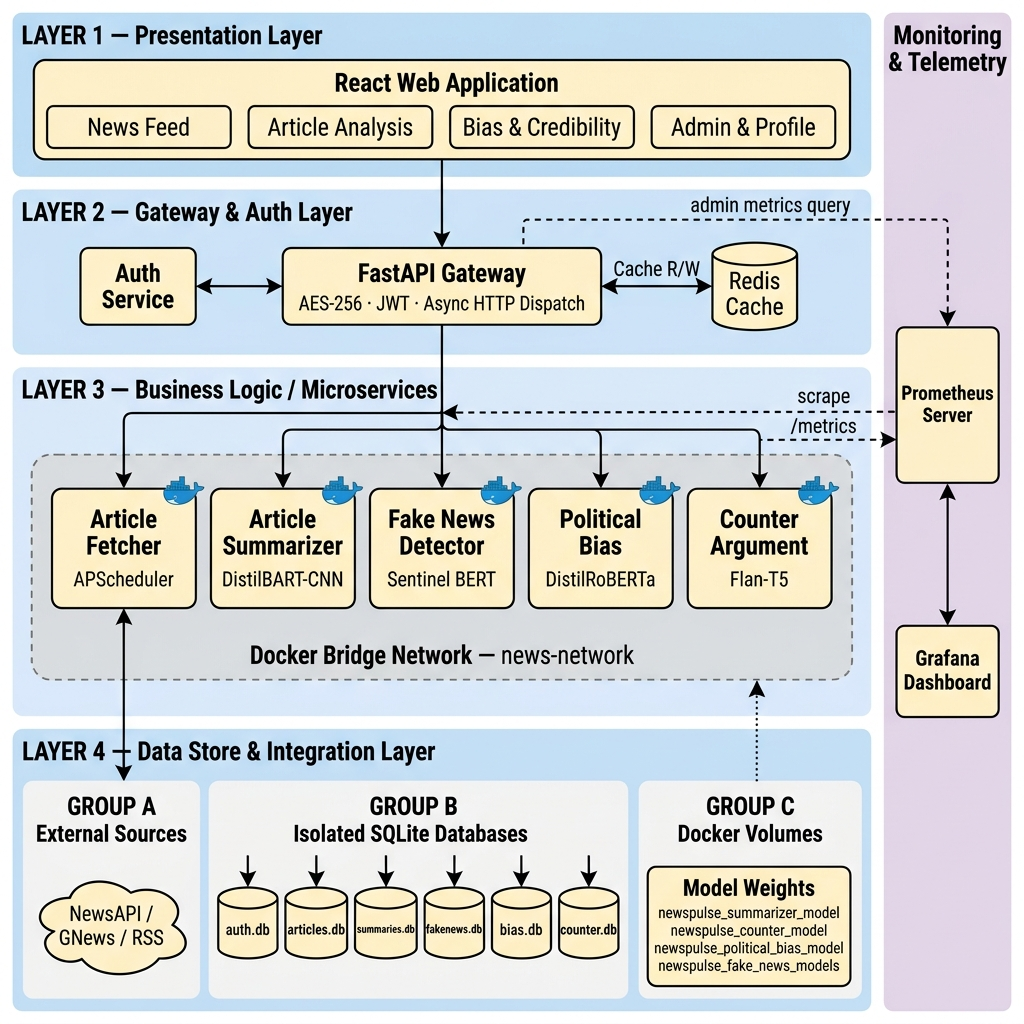
\includegraphics[width=1\linewidth]{BS_FYP_Figs/architecture_diagram.png}
    \caption{Architecture Diagram illustrating the 11-node microservices topology}
    \label{fig:architecture-diagram}
\end{figure}

As shown in Figure~\ref{fig:architecture-diagram}, the NewsPulse system is structured as an 11-node microservices topology divided into three primary tiers:
\begin{itemize}
    \item \textbf{Presentation Tier:} A single React-based single-page application (SPA) container running on port 3000 (mapped to port 80 inside Nginx). This tier renders the vector visualization dashboards and executes client-side cryptographic functions.
    \item \textbf{Gateway and Coordination Tier:} A central FastAPI Gateway container (port 8000) that serves as the single point of entry. It is allocated a resource boundary of 2.0 CPUs and 2 GB of RAM. The gateway decrypts incoming payloads using its private RSA-2048 key, performs user validation, checks JWT access tokens, and aggregates the multi-signal downstream results. It interfaces with an in-memory Redis caching container (port 6379, limited to 1.0 CPU and 2 GB of RAM) running `redis:7.4-alpine` to prevent duplicate inference passes.
    \item \textbf{Computational NLP Tier:} A suite of stateless FastAPI microservices operating within private Docker container environments:
    \begin{itemize}
        \item \texttt{article\_summarizer}: Bound to port 8001 (internal port 8000) with a limit of 4.0 CPUs and 8 GB of RAM. It generates summaries using a local instance of the \texttt{sshleifer/distilbart-cnn-12-6} model, storing weights in the persistent \texttt{newspulse\_summarizer\_model} volume.
        \item \texttt{fakenews\_detection}: Bound to port 8005 (internal port 8000) with a limit of 4.0 CPUs and 6 GB of RAM. It implements the Sentinel consensus algorithm, combining deep learning sequence classification from a local \texttt{dhruvpal/fake-news-bert} model with custom stylometric heuristics.
        \item \texttt{political\_bias}: Bound to port 8003 (internal port 8000) with a limit of 4.0 CPUs and 6 GB of RAM. It runs the \texttt{valurank/distilroberta-bias} model over overlapping sliding windows.
        \item \texttt{counter\_argument}: Bound to port 8002 (internal port 8000) with a limit of 2.0 CPUs and 4 GB of RAM. It generates critical perspectives using a PyTorch quantized \texttt{MBZUAI/LaMini-Flan-T5-248M} model, with \texttt{google/flan-t5-base} as a fallback.
    \end{itemize}
    \item \textbf{Ingestion Tier:} The \texttt{article\_fetcher} daemon container (port 8004) running with 1.0 CPU and 2 GB of RAM. It executes a background non-blocking aggregation loop every 15 minutes, scraping articles from public API feeds and RSS channels.
    \item \textbf{Telemetry Tier:} Comprises isolated Prometheus (port 9090) and Grafana (port 3001) containers. These services scrape operational metrics from the FastAPI \texttt{/metrics} endpoints to generate time-series dashboards.
\end{itemize}

\section{Domain Model Diagram}
The Domain Model establishes the vocabulary and logical boundaries of the computational journalism entities. The primary \texttt{Article} entity acts as the central node, correlating with specialized intelligence components including \texttt{Summarization}, \texttt{FakeNewsDetection}, \texttt{BiasedAnalysis}, and \texttt{CounterArgument}. These domain relationships map directly to the respective NLP pipelines rather than a centralized database, maintaining the principles of domain-driven design.

\begin{figure}[h!]
    \centering
    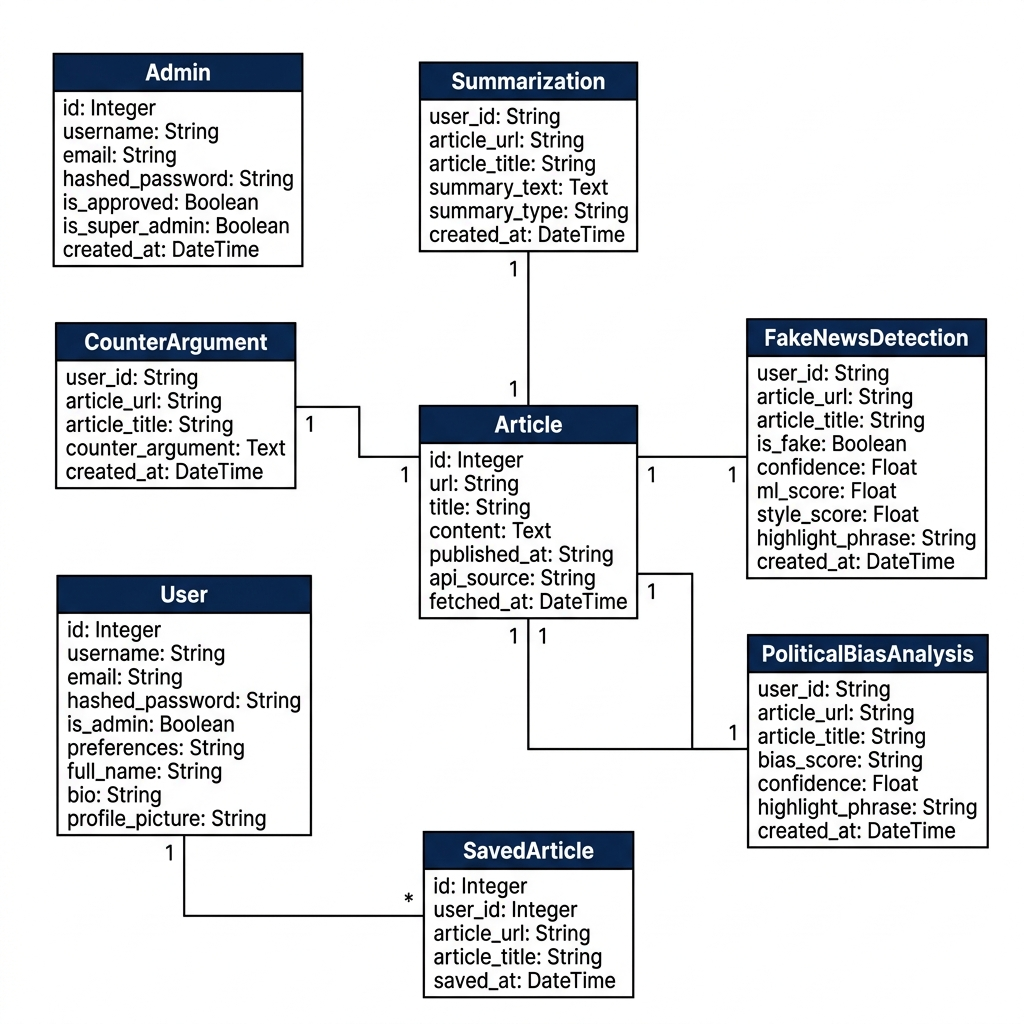
\includegraphics[width=1\linewidth]{BS_FYP_Figs/domain_model_diagram.png}
    \caption{Domain Model Diagram representing core intelligence entities}
    \label{fig:domain-model-diagram}
\end{figure}

The domain boundaries, modeled in Figure~\ref{fig:domain-model-diagram}, enforce a "Shared-Nothing" data architecture. The \texttt{Article} entity is represented as a self-contained, immutable aggregate containing raw text content, publication timestamps, category classifications, and publisher domain data. This aggregate is passed as an isolated payload across the microservices. 

Rather than relying on a centralized database that links reports via foreign keys, each analytical outcome is treated as a distinct, value-object component. For example, \texttt{Summarization} contains only the abstractive text output and processing latency, while \texttt{FakeNewsDetection} encapsulates stylometric density signals, ML probability scores, and XAI sentence highlights. This design ensures that each container remains completely autonomous, allowing changes to one analytical domain model to be made without modifying the structures of adjacent containers.

\section{Entity Relationship Diagram}
To strictly enforce microservice decoupling, the system avoids cross-service foreign key dependencies. The Entity Relationship Diagram details isolated SQLite clusters. The \texttt{auth\_service} schema contains independent \texttt{Users}, \texttt{Admins}, and \texttt{SavedArticles} tables utilizing \texttt{passlib} bcrypt hashing. Concurrently, individual AI microservices maintain localized history tables to log inference queries for localized auditing and telemetry extraction.

\begin{figure}[h!]
    \centering
    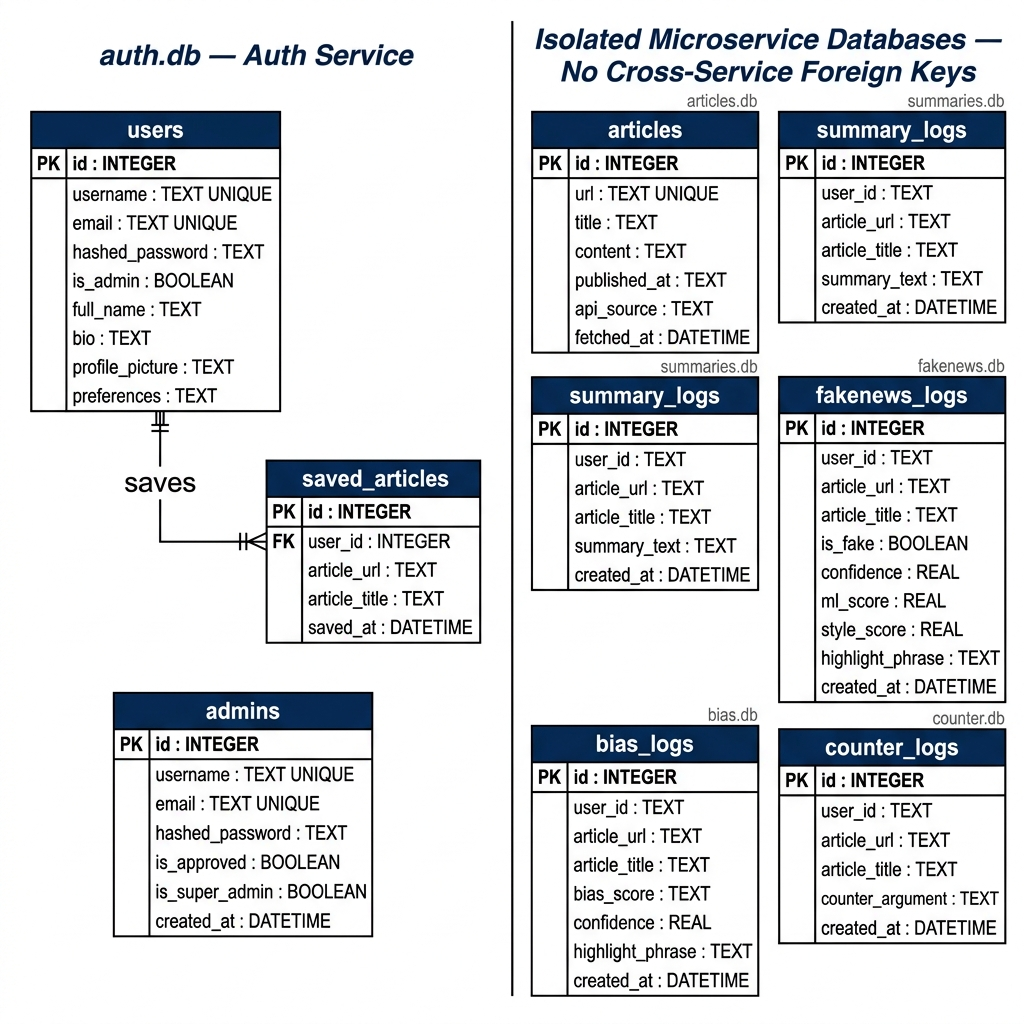
\includegraphics[width=0.9\linewidth]{BS_FYP_Figs/er_diagram.png}
    \caption{Entity Relationship Diagram detailing isolated microservice database schemas}
    \label{fig:entity-relationship-diagram}
\end{figure}

To prevent tight database coupling, the ERD modeled in Figure~\ref{fig:entity-relationship-diagram} uses isolated SQLite database instances running in separate Docker container volumes. 
\begin{itemize}
    \item \textbf{Authentication Service Schema:} Contains three core tables:
    \begin{itemize}
        \item \texttt{Users}: Stores user authentication records, including emails and password hashes generated using \texttt{passlib}'s \texttt{bcrypt} implementation.
        \item \texttt{Admins}: Stores operational administrator configurations for metrics validation.
        \item \texttt{SavedArticles}: Saves forensic reports generated by users, storing summaries, credibility consensus scores, bias ratings, and Socratic counter-arguments along with a dynamic article hash.
    \end{itemize}
    \item \textbf{AI Microservice Logging Schemas:} Each computational container (summarization, bias, credibility, and debate) maintains an isolated local SQLite logging table. These tables record operational metadata, including request text hashes, processing times, loaded model weights, memory usage, and execution outcomes. This localized design allows audits and telemetry queries to run without impacting the security boundaries of user credentials.
\end{itemize}

\section{Class Diagram}
The Object-Oriented structure within the localized FastAPI containers utilizes Pydantic data validation and localized pipeline classes. The Class Diagram highlights the implementation of the \texttt{SocraticDebaterEngine} utilizing regex templates, the \texttt{TopicGate} penalty class for bias suppression, and the \texttt{ConsensusFakeNewsDetector} class which computes the weighted average of the \texttt{fake-news-bert} output against stylometric density heuristics.

\begin{figure}[h!]
    \centering
    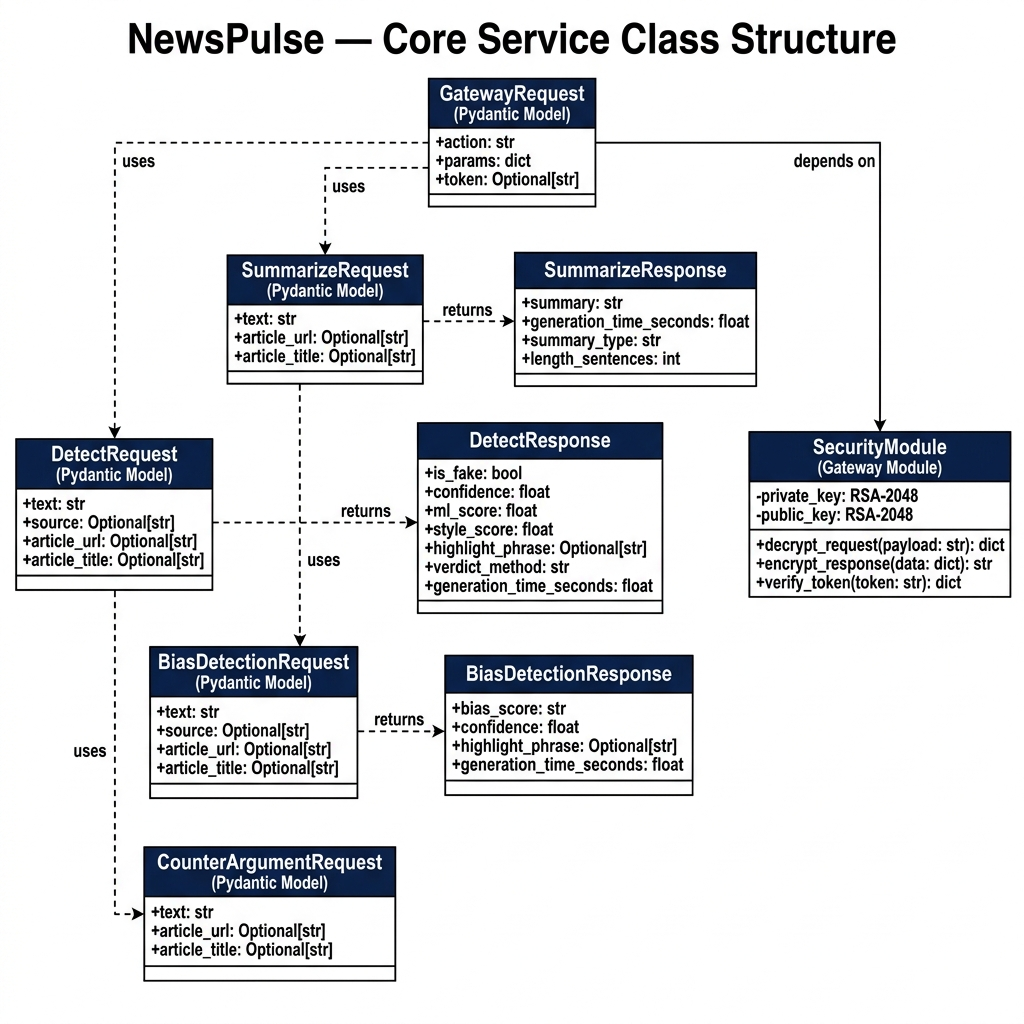
\includegraphics[width=1\linewidth]{BS_FYP_Figs/class_diagram.png}
    \caption{Class Diagram mapping Pydantic models and deterministic NLP pipelines}
    \label{fig:class-diagram}
\end{figure}

The class structure of the computational pipelines, as illustrated in Figure~\ref{fig:class-diagram}, relies on \texttt{Pydantic} validation classes to enforce strict type checking and data validation at runtime:
\begin{itemize}
    \item \textbf{Validation Classes:} \texttt{ArticleRequest} validates input fields, enforcing length boundaries and content limits. \texttt{AnalysisResponse} validates outgoing payloads, ensuring all analytical outputs are complete before encryption.
    \item \textbf{ConsensusFakeNewsDetector Class:} Implements the Sentinel engine. It coordinates the \texttt{DHruvPalFakeNewsBERT} wrapper, the \texttt{StylometricHeuristics} class (which computes sensationalism and capitalization ratios), and the \texttt{CognitiveComplexity} evaluator. It combines these metrics with live API fact-checking adjustments and objective style caps to calculate the final credibility consensus.
    \item \textbf{PoliticalBiasClassifier Class:} Manages DistilRoBERTa bias evaluations using the \texttt{WindowAverager} helper. It coordinates the \texttt{TopicGate} class, which applies apolitical keyword penalties to force bias ratings to "Center" in apolitical domains.
    \item \textbf{SocraticDebaterEngine Class:} Wraps the PyTorch quantized Flan-T5 model. It uses post-processing filters to clean generated counter-arguments and executes the template-based proper-noun lookup fallback if the sequence generation times out.
\end{itemize}

\section{Activity Diagram}
The system activity flow governs the concurrent execution of multi-signal AI inferences. Upon receiving an encrypted payload, the gateway validates the JSON Web Token (JWT) and checks the Redis caching broker. On a cache miss, the system executes parallel requests to the summarizer, bias detector, and fake news microservices. The activity concludes by aggregating the outputs, symmetrically encrypting the response, and returning the forensic data to the React frontend.

\begin{figure}[h!]
    \centering
    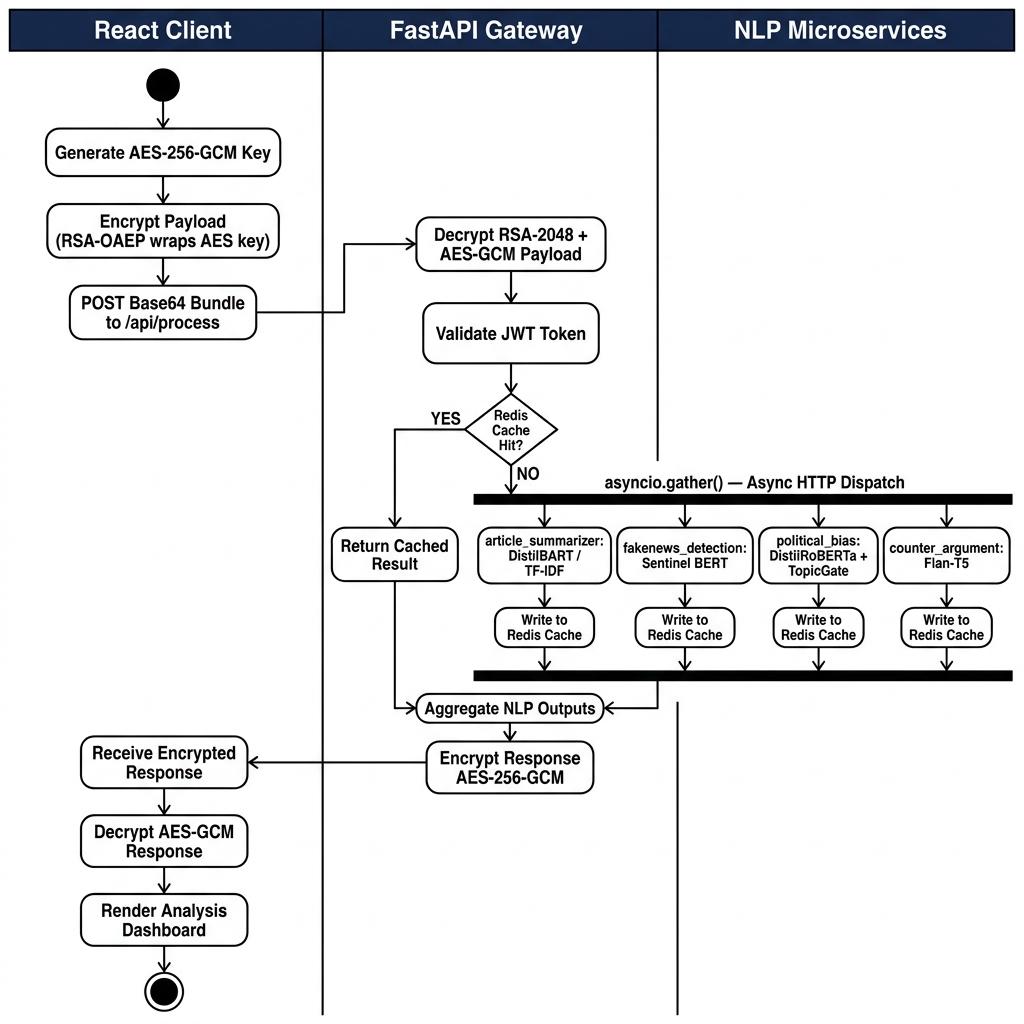
\includegraphics[width=0.6\linewidth]{BS_FYP_Figs/activity_diagram.jpg}
    \caption{Activity Diagram detailing concurrent NLP pipeline execution and caching}
    \label{fig:activity-diagram}
\end{figure}

The execution sequence modeled in Figure~\ref{fig:activity-diagram} coordinates request validation, caching checks, and concurrent inference pipelines:
\begin{enumerate}
    \item The React client encrypts request parameters using AES-256-GCM and transmits the Base64-encoded payload to the API Gateway.
    \item The gateway decrypts the payload using its private RSA key and validates the JWT.
    \item The gateway hashes the input text using SHA-256 and queries Redis. If a cached analysis is found, the gateway immediately returns the cached result to the client.
    \item If the query misses the cache, the gateway uses a \texttt{ThreadPoolExecutor} to invoke the four computational NLP containers in parallel.
    \item The microservices process the request simultaneously: \texttt{article\_summarizer} truncates input to 2500 characters and generates a summary; \texttt{fakenews\_detection} evaluates credibility; \texttt{political\_bias} determines polarization; and \texttt{counter\_argument} generates counter-arguments.
    \item The gateway aggregates these outputs, writes the combined result to Redis, encrypts the payload using AES-256-GCM, and returns the response to the client.
\end{enumerate}

\section{State Transition Diagram}
The State Transition Diagram defines the system's structural resilience mechanisms when operating under severe hardware constraints. It models the critical fallback states: navigating from standard API aggregation to \texttt{trafilatura} web scraping upon payload truncation, and degrading from the memory-intensive \texttt{distilbart-cnn-12-6} transformer state to a deterministic Term Frequency-Inverse Document Frequency (TF-IDF) extraction state during out-of-memory (OOM) anomalies.

\begin{figure}[h!]
    \centering
    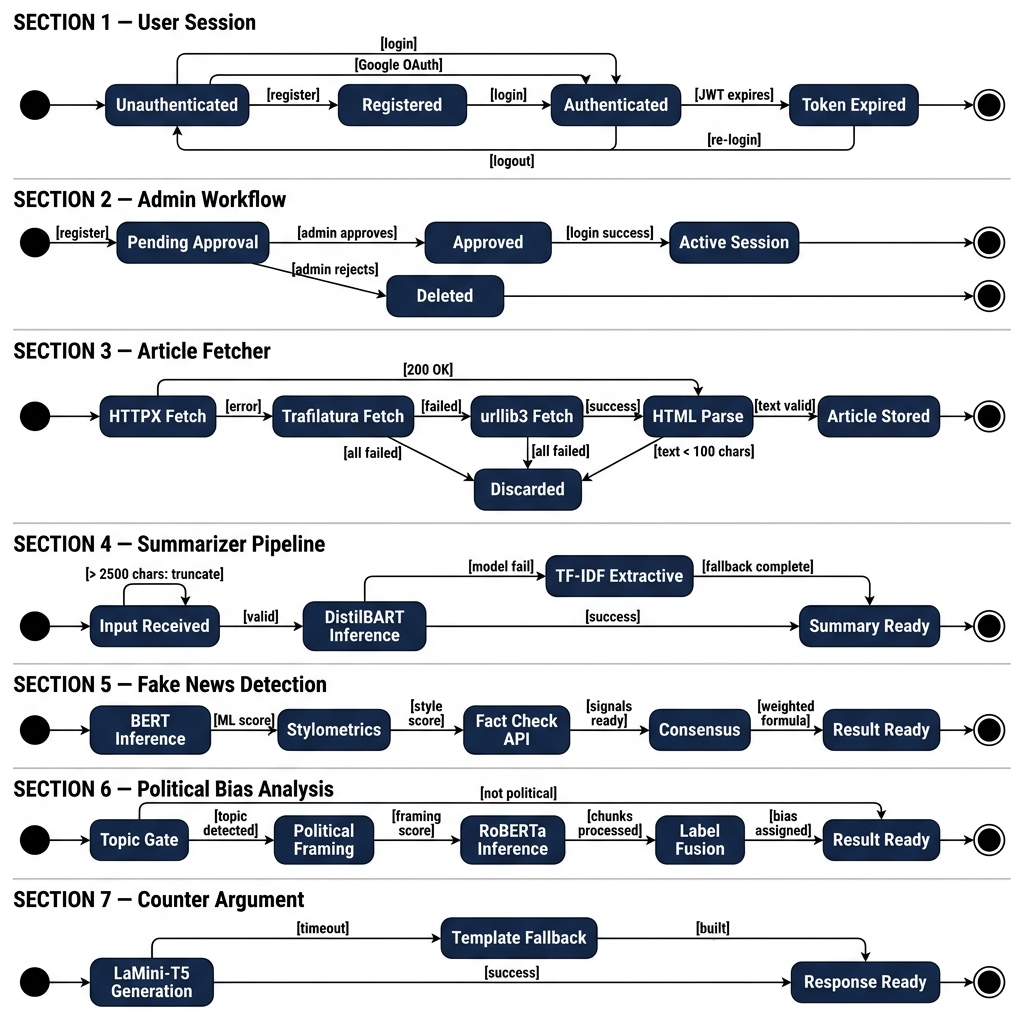
\includegraphics[width=0.7\linewidth]{BS_FYP_Figs/state_transition_diagram.png}
    \caption{State Transition Diagram defining heuristic degradation and fallback mechanisms}
    \label{fig:state-transition-diagram}
\end{figure}

As shown in Figure~\ref{fig:state-transition-diagram}, the system shifts through explicit operating states to maintain availability under heavy workloads:
\begin{itemize}
    \item \textbf{Ingestion Scraping States:} The \texttt{article\_fetcher} starts in a \texttt{Standard\_API\_Aggregation} state. If blocked or if RSS feeds are incomplete, it transitions to a \texttt{Spoofed\_HTTPX\_Request} state. If anti-bot shields are encountered, it shifts to a \texttt{Trafilatura\_Extraction} state. If TLS connection blocks occur, it degrades to a \texttt{Bypassed\_SSL\_urllib3} socket state before discarding incomplete text under 100 characters.
    \item \textbf{Summarizer Operating States:} The summarization microservice starts in a \texttt{DistilBART\_Deep\_Inference} state. If the input exceeds the 2500-character safety limit, the system truncates the text to prevent memory errors. If memory is depleted or pipeline execution fails, the service shifts to a \texttt{Deterministic\_TF\_IDF\_Extraction} fallback state.
    \item \textbf{Socratic Debater States:} The debater starts in a \texttt{Quantized\_Flan\_T5\_Generation} state. If sequence generation times out or loops are detected, the system transitions to a \texttt{Proper\_Noun\_Domain\_Template} state, using regex and pre-defined academic templates to construct a counter-argument.
\end{itemize}

\section{Component Diagram}
The structural modules driving the application logic are mapped in the Component Diagram. The frontend utilizes \texttt{@react-oauth/google} and \texttt{recharts} for data visualization. The security component integrates \texttt{node-forge} and Python's \texttt{cryptography} module for AES-GCM processing. Background operations are encapsulated within an \texttt{APScheduler} and \texttt{ThreadPoolExecutor} component to handle asynchronous hyper-text markup language (HTML) parsing without blocking the primary event loops.

\begin{figure}[h!]
    \centering
    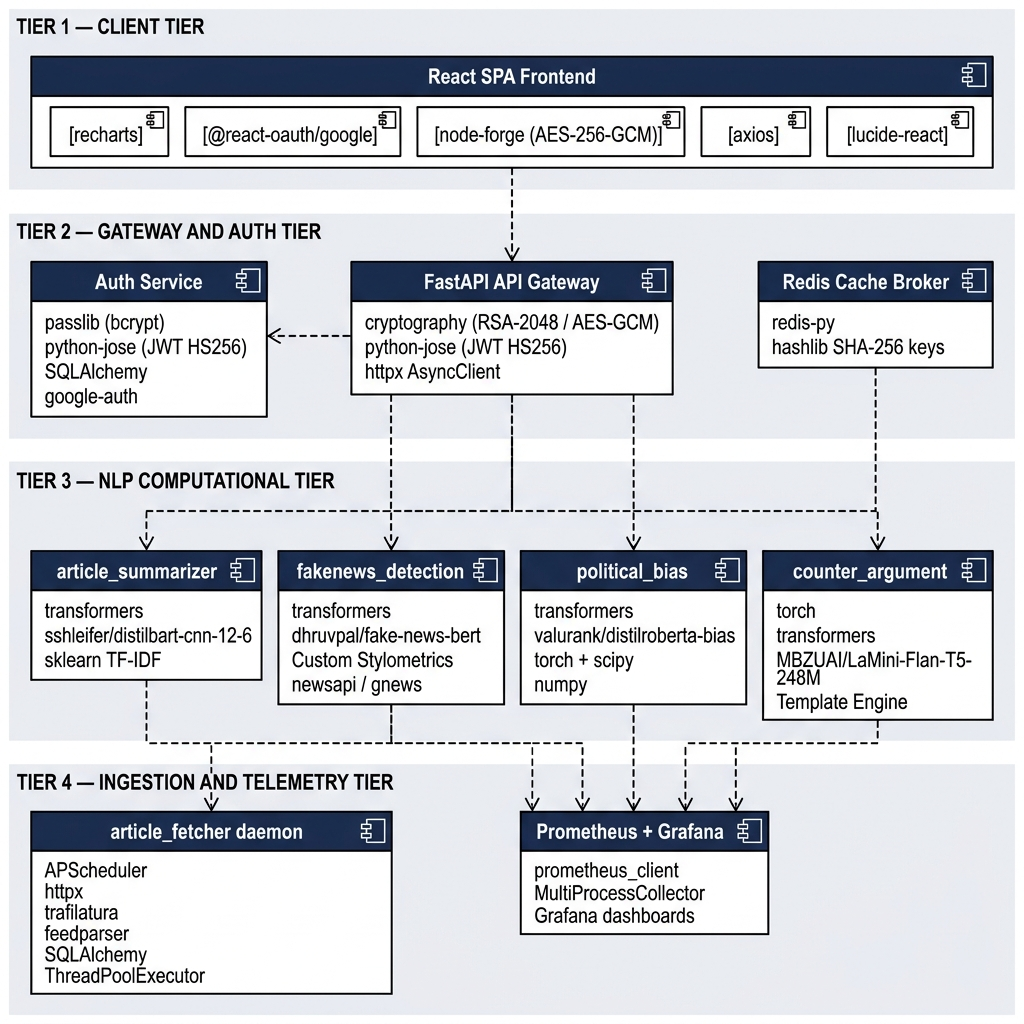
\includegraphics[width=1\linewidth]{BS_FYP_Figs/component_diagram.png}
    \caption{Component Diagram outlining explicit library dependencies and software modules}
    \label{fig:component-diagram}
\end{figure}

The Component Diagram modeled in Figure~\ref{fig:component-diagram} defines the library dependencies and internal packages that drive each microservice:
\begin{itemize}
    \item \textbf{Frontend Presentation Module:} Coordinates two key subcomponents:
    \begin{itemize}
        \item \texttt{@react-oauth/google}: Standard Google identity provider integration.
        \item \texttt{recharts}: Vector graphing module that renders polarization and credibility metrics.
    \end{itemize}
    \item \textbf{Cryptographic Security Module:} Integrates the Javascript library \texttt{node-forge} on the client side and the standard Python \texttt{cryptography} library on the gateway. These packages manage RSA-OAEP public-key encryption and symmetric AES-256-GCM data encryption.
    \item \textbf{Ingestion Ingestion Module:} Uses spoofed async requests and \texttt{trafilatura} to extract text, coordinate async fetch loops, and run title deduplication.
    \item \textbf{Computational NLP Modules:} Integrate PyTorch wrappers and HuggingFace pipelines. The debater service uses PyTorch's dynamic quantization (\texttt{torch.quantization.quantize\_dynamic}) to optimize model weights for CPU execution.
\end{itemize}

\section{Deployment Diagram}
The deployment infrastructure requires zero reliance on proprietary cloud Graphical Processing Units (GPUs). The React presentation layer is deployed to a static edge network (Vercel). The FastAPI and Docker Compose backend stack executes on localized commercial off-the-shelf (COTS) hardware, utilizing Ngrok or Cloudflare Tunnels to securely expose the internal gateway port (8000) to the public internet.

\begin{figure}[h!]
    \centering
    \includegraphics[width=0.4\linewidth]{BS_FYP_Figs/deployement_diagram.png}
    \caption{Deployment Diagram modeling hybrid edge and tunneled localhost hosting}
    \label{fig:deployment-diagram}
\end{figure}

The deployment topology illustrated in Figure~\ref{fig:deployment-diagram} is designed for local hosting on consumer off-the-shelf (COTS) hardware, eliminating the need for expensive GPU cloud instances:
\begin{itemize}
    \item \textbf{Presentation Layer Deployment:} The static React Single Page Application is hosted on Vercel's global edge network, ensuring fast page load times and global reach.
    \item \textbf{On-Premise Computational Host:} The backend services are deployed on a local server running a standard Linux kernel. A Docker Compose runtime hosts the 11 isolated containers, separated from external network traffic by a private bridge network.
    \item \textbf{Secure Transit Tunneling:} An \texttt{ngrok} or Cloudflare daemon runs in the background. It establishes a secure, outbound HTTPS tunnel that binds the internal gateway port (8000) to a public URL. This setup allows the client application to communicate securely with the local gateway without requiring public IP configurations.
\end{itemize}

\section{Data Flow Diagram}
The Data Flow Diagram (DFD) maps the trajectory of secure information exchange and system telemetry. It traces the End-to-End Payload Encryption, where the React client encrypts data utilizing a public RSA-OAEP key (\texttt{public\_key.pem}). Furthermore, it maps the flow of internal hardware metrics from the \texttt{prometheus\_client.multiprocess.MultiProcessCollector} across multiple Gunicorn/Uvicorn workers directly into the Grafana visualization dashboard.

\begin{figure}[h!]
    \centering
    
\includegraphics[width=1\linewidth]{BS_FYP_Figs/data_flow_diagram.png}
    \caption{Data Flow Diagram tracking AES-GCM encryption and Prometheus telemetry}
    \label{fig:data-flow-diagram}
\end{figure}

The DFD modeled in Figure~\ref{fig:data-flow-diagram} traces the flow of data through the system, focusing on cryptographic transit and telemetry collection:
\begin{itemize}
    \item \textbf{Cryptographic Transit Path:} 
    \begin{enumerate}
        \item The React client generates a dynamic 32-byte AES key and encrypts the plaintext request using AES-256-GCM.
        \item The client encrypts the AES key using the gateway's public RSA-2048 key.
        \item The encrypted key (first 256 bytes), IV (16 bytes), ciphertext, and tag (last 16 bytes) are base64-encoded and sent to the gateway.
        \item The gateway decrypts the payload, processes the request through the NLP microservices, and returns a symmetrically encrypted response.
    \end{enumerate}
    \item \textbf{Telemetry Metrics Collection Path:}
    \begin{enumerate}
        \item Individual microservice containers collect operational performance data using the Python \texttt{prometheus\_client} library.
        \item To monitor multi-worker environments, the collector writes worker thread statistics to a shared multiprocess directory using \texttt{MultiProcessCollector}.
        \item The Prometheus scraper polls the \texttt{/metrics} endpoint of each service and writes the metrics to its time-series database.
        \item Grafana queries Prometheus and displays real-time system performance, CPU metrics, and cache hit ratios on dashboards.
    \end{enumerate}
\end{itemize}
